\section{Gleichstrommaschine im Umrichterbetrieb}

Diese Section behandelt die \textbf{Gleichstrommaschine} als Last und Antrieb
im Zusammenspiel mit Gleichrichtern und Gleichstromstellern.
Sie ist zentral für die Analyse von \textbf{Drehzahl}, \textbf{Drehmoment}, \textbf{Stabilität}
und für das Verständnis der \textbf{Kennlinien $M$–$n$}.

\smallskip

\textbf{Zielbild:}
\begin{itemize}
    \item Grundgleichungen der Gleichstrommaschine kennen
    \item Zusammenhang zwischen Spannung, Strom, Drehzahl und Drehmoment verstehen
    \item Einfluss der Ankerspannung auf die Drehzahl analysieren
    \item Stabilen und instabilen Betrieb beurteilen
\end{itemize}

\subsection{Grundaufbau und Ersatzschaltbild}
\begin{center}
    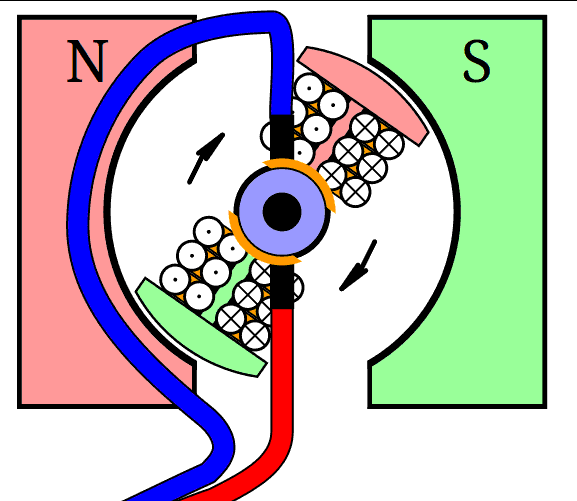
\includegraphics[width=0.85\linewidth]{images/Grundaufbau_gleistrommaschiene.png}
\end{center}
\subsubsection{Vereinfachtes Ersatzschaltbild}

\begin{center}
    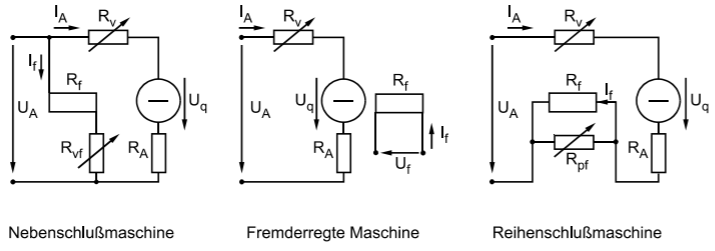
\includegraphics[width=0.85\linewidth]{images/gleichstrommasciene.png}
\end{center}

\textbf{Elemente:}
\begin{itemize}
    \item $u_a(t)$: Ankerspannung aus Umrichter oder Steller
    \item $R_a$: Ankerwiderstand
    \item $L_a$: Ankerinduktivität
    \item $E_i$: induzierte Gegenspannung
    \item $i_a(t)$: Ankerstrom
\end{itemize}

\subsection{Grundgleichungen der Gleichstrommaschine}

\subsubsection{Elektrische Gleichung}

\[
\cbl{u_a(t) = R_a\, i_a(t) + L_a\, \frac{di_a(t)}{dt} + E_i(t).}
\]

\subsubsection{Gegenspannung}

Die induzierte Gegenspannung ist proportional zur Drehzahl:
\[
\cbl{E_i = k_e \, \omega = \omega \, \Psi.}
\]

Dabei:
\begin{itemize}
    \item $\omega$: mechanische Winkelgeschwindigkeit
    \item $\Psi$: Erregerfluss
\end{itemize}

\subsubsection{Drehmomentgleichung}

Das elektromagnetische Drehmoment ist proportional zum Ankerstrom:
\[
\cbl{M = k_m \, i_a = i_a \, \Psi.}
\]

\crd{\textrightarrow\ Drehmoment wird \textbf{direkt durch den Strom} bestimmt.}

\subsection{Mechanische Gleichung}

Die mechanische Bewegungsgleichung lautet:
\[
\cbl{J \frac{d\omega}{dt} = M - M_L - B\,\omega.}
\]

Dabei:
\begin{itemize}
    \item $J$: Trägheitsmoment
    \item $M_L$: Lastmoment
    \item $B$: Reibungskoeffizient
\end{itemize}

Im stationären Betrieb gilt:
\[
M = M_L.
\]

\subsection{Stationärer Betrieb}

Im stationären Gleichgewicht:
\[
\frac{di_a}{dt} = 0, \qquad \frac{d\omega}{dt} = 0.
\]

Damit:
\[
\cbl{u_a = R_a\, i_a + E_i = R_a\, i_a + \omega \Psi.}
\]

Auflösen nach der Drehzahl:
\[
\cbl{\omega = \frac{u_a - R_a i_a}{\Psi}.}
\]

Interpretation:
\begin{itemize}
    \item Drehzahl steigt mit Ankerspannung.
    \item Drehzahl sinkt mit wachsendem Laststrom.
\end{itemize}

\subsection{M--n-Kennlinie (Drehmoment-Drehzahl-Kennlinie)}

Kombination aus:
\[
M = i_a \Psi, \qquad
\omega = \frac{u_a - R_a i_a}{\Psi}.
\]

Elimination von $i_a$:
\[
\cbl{\omega = \frac{u_a}{\Psi} - \frac{R_a}{\Psi^2} M.}
\]

Das ist eine \textbf{lineare Kennlinie}.



\textbf{Kennwerte:}
\begin{itemize}
    \item Leerlaufdrehzahl:
    \[
    \cbl{\omega_0 = \frac{u_a}{\Psi}}
    \]
    \item Kurzschlussmoment:
    \[
    \cbl{M_K = \frac{u_a \Psi}{R_a}}
    \]
\end{itemize}

\subsection{Dynamisches Modell der Gleichstrommaschine}

Mechanische Bewegungsgleichung:
\[
\boxed{J \frac{d\omega}{dt} = M - M_L}
\]

Elektrische Gleichung:
\[
\boxed{u_a = R_a i_a + L_a \frac{di_a}{dt} + k\Phi \omega}
\]

Das System ist ein gekoppeltes elektrisches–mechanisches System.

\subsection{Einfluss der Ankerspannung}

Für verschiedene $u_a$ entstehen parallele Kennlinien:

\textbf{Aussage:}
\begin{itemize}
    \item Spannungsregelung $\Rightarrow$ Drehzahlregelung.
    \item Steigung bleibt konstant, nur Achsenabschnitt ändert sich.
\end{itemize}

\subsection{Arbeitspunkt und Stabilität}

Der Arbeitspunkt ist der Schnittpunkt von:
\begin{itemize}
    \item Motorkennlinie $\omega(M)$
    \item Lastkennlinie $\omega_L(M)$
\end{itemize}

\subsection{Skizze 2: Stabiler Arbeitspunkt}



Stabilitätskriterium:
\[
\cbl{\frac{d\omega_M}{dM} < \frac{d\omega_L}{dM} \quad \Rightarrow \text{stabil}.}
\]

\crd{\textrightarrow\ Bei falscher Steigung entsteht \textbf{instabiler Betrieb}.}

\subsection{Einfluss des Erregerflusses}

Bei veränderlichem Fluss $\Psi$:

\[
\omega_0 = \frac{u_a}{\Psi}, \qquad M = i_a \Psi.
\]

\begin{itemize}
    \item Feldschwächung ($\Psi \downarrow$) $\Rightarrow$ Drehzahl steigt.
    \item Drehmomentfähigkeit sinkt.
\end{itemize}

\subsection{Zusammenhang mit dem Umrichter}

Bei Betrieb am Gleichrichter oder Gleichstromsteller:
\[
\cbl{u_a = \overline{u_2} = d \, U_{\mathrm{DC}} \quad \text{oder} \quad \frac{2\hat U}{\pi} \cos(\alpha).}
\]

Damit:
\begin{itemize}
    \item Drehzahl direkt steuerbar über $d$ oder $\alpha$.
    \item Strom bestimmt das Drehmoment.
\end{itemize}

\subsection{Typische Merksätze (Prüfungskern)}

\begin{itemize}
    \item $E_i = \omega \Psi$
    \item $M = i_a \Psi$
    \item $\omega = \dfrac{u_a - R_a i_a}{\Psi}$
    \item M--n-Kennlinie ist linear.
    \item Drehmoment wird über Strom geregelt.
\end{itemize}

\subsection{Typische Fehlerquellen}

\begin{itemize}
    \item Gegenspannung vergessen.
    \item Drehmoment mit Spannung statt mit Strom verknüpft.
    \item Stabilitätskriterium falsch interpretiert.
    \item Feldfluss als konstant angenommen, obwohl Feldschwächung vorliegt.
\end{itemize}

\subsection{Minimal-Checkliste für Aufgaben}

\begin{enumerate}
    \item Ankerspannung $u_a$ bestimmen.
    \item Gegenspannung $E_i = \omega \Psi$ ansetzen.
    \item Strom aus $u_a = R_a i_a + E_i$ berechnen.
    \item Drehmoment $M = i_a \Psi$ berechnen.
    \item Arbeitspunkt aus Schnitt Motor–Last bestimmen.
    \item Stabilität qualitativ prüfen.
\end{enumerate}
\subsection{Schnellentscheidungshilfen für die Gleichstrommaschine}

Diese Merksätze erlauben eine schnelle qualitative Beurteilung in Prüfungsaufgaben.

\paragraph{Grundgleichungen}

\[
u_a = R_a i_a + k\Phi \omega
\]
\[
M = k\Phi i_a
\]

\paragraph{Einfluss der Ankerspannung $u_a$}

\begin{itemize}
\item $u_a \uparrow \;\Rightarrow\; \omega \uparrow$
\item $u_a \downarrow \;\Rightarrow\; \omega \downarrow$
\item $u_a = 0 \;\Rightarrow\; \omega = 0$ (Stillstand)
\end{itemize}

\paragraph{Einfluss des Lastmoments $M_L$}

\begin{itemize}
\item $M_L \uparrow \;\Rightarrow\; i_a \uparrow \;\Rightarrow\; \omega \downarrow$
\item $M_L \downarrow \;\Rightarrow\; i_a \downarrow \;\Rightarrow\; \omega \uparrow$
\end{itemize}

\paragraph{Einfluss des Erregerflusses $\Phi$}

\begin{itemize}
\item $\Phi \uparrow \;\Rightarrow\; \omega \downarrow$ (Feldschwächung umgekehrt)
\item $\Phi \downarrow \;\Rightarrow\; \omega \uparrow$
\item $\Phi \downarrow \;\Rightarrow\; M_{\max} \downarrow$
\end{itemize}

\paragraph{Motoranlauf}

Beim Anlauf gilt:
\[
\omega = 0 \;\Rightarrow\; E = k\Phi \omega = 0
\]

Damit:
\[
\boxed{i_{a,0} = \frac{u_a}{R_a}}
\]

Konsequenzen:
\begin{itemize}
\item Sehr hoher Anlaufstrom.
\item Anlaufwiderstand oder Stromregelung notwendig.
\item Drehmoment beim Anlauf:
\[
\boxed{M_0 = k\Phi i_{a,0}}
\]
\end{itemize}

\paragraph{Typische Prüfungsfragen}

\begin{itemize}
\item $u_a$ erhöhen $\Rightarrow$ Drehzahl steigt.
\item Lastmoment steigt $\Rightarrow$ Strom steigt, Drehzahl sinkt.
\item Feldschwächung $\Rightarrow$ hohe Drehzahl, kleines Drehmoment.
\item Beim Anlauf ist der Strom maximal.
\end{itemize}

\crd{\textrightarrow\ Diese Merksätze erlauben schnelle qualitative Entscheidungen ohne Rechnung.}

